\documentclass[aspectratio=169, hyperref={pdfpagelabels=false}]{beamer}
%\usepackage{helvet}
%\renewcommand{\familydefault}{\rmdefault}
%\usepackage{mathpazo}
\usepackage{newpxmath}
\usefonttheme{professionalfonts}
\usefonttheme{serif}
\usepackage[english]{babel}
\usepackage{pgfplots}
\usepackage{pgf}
\usepackage{pgfpages}
\pgfplotsset{compat=newest}
\usepackage{booktabs}
\usepackage[T1]{fontenc}
\usepackage[utf8]{inputenc}
\usepackage{lipsum}
\usepackage{tcolorbox}
\usepackage{xcolor}
\usepackage{listings}
\usepackage{microtype}
\usepackage{float}
\usepackage{siunitx}
\usepackage{multicol}
\usepackage{hyperref}
\usepackage{dsfont}
\usepackage{caption}
\usepackage{subcaption}
\usepackage{dashbox}
\usepackage{csquotes}
\usepackage[absolute, overlay]{textpos}
\usepackage{trfrac}

\setlength{\TPHorizModule}{\textwidth}
\setlength{\TPVertModule}{\textwidth}

\input{template/settings}

\newcommand{\setcolor}[1]{\def\chosencolor{#1}}
\newcommand{\setdepartment}[1]{\def\department{#1}}

\DeclareMathOperator*{\argmax}{argmax}
\DeclareMathOperator*{\argmin}{argmin}
\DeclareMathOperator{\E}{\mathbb{E}}

\newcommand{\indep}{\perp \!\!\! \perp}

\usetheme{DTU}
\setbeamersize{text margin left=22mm}
\def\insertframetitle{}

\newcommand{\inserttitlepage}{
    \begin{frame}[plain, noframenumbering]{}

        \begin{center}
        \hspace{-3.6em}
            \includegraphics[width = 0.25\paperwidth]{logos/\targetcolourmodel/white.pdf}
        \end{center}
        
    \end{frame}

    \begin{frame}[plain]{}
        \color{white}\maketitle
    \end{frame}

    \setbeamercolor{background canvas}{bg = white}
}


%\AtBeginSection[]{
%  \begin{frame}[plain, noframenumbering]{}
%        %\usebeamercolor[fg]{title}
%        
%        % title
%               {\Large\insertsubtitle\par}\vspace{2mm}
%               {\usebeamerfont{title}\textbf{\insertsectionhead\par}\par}\vspace{5mm}
%               {\Large\insertauthor\par}\vspace{5mm}
%  \end{frame}
%    }





%% Algorithm
\newcounter{nalg} % defines algorithm counter
\renewcommand{\thenalg}{\arabic{nalg}} %defines appearance of the algorithm counter
\DeclareCaptionLabelFormat{algocaption}{Algorithm \thenalg} % defines a new caption label as Algorithm x.y
\definecolor{cadet}{rgb}{0.33, 0.41, 0.47}
\lstnewenvironment{algorithm}[1][] %defines the algorithm listing environment
{   
    \refstepcounter{nalg} %increments algorithm number
    \captionsetup{labelformat=algocaption,labelsep=colon} %defines the caption setup for: it ises label format as the declared caption label above and makes label and caption text to be separated by a ':'
    \lstset{ %this is the stype
        mathescape=true,
        frame=tB,
        numbers=left, 
        numberstyle=\tiny,
        basicstyle=\scriptsize\ttfamily, 
        keywordstyle=\color{black}\bfseries,
        keywords={,optional, input, output, return, datatype, function, if, else, for, foreach, begin, end, } %add the keywords you want, or load a language as Rubens explains in his comment above.
        numbers=left,
        xleftmargin=.04\textwidth,
        morecomment=[l][\color{cadet}]{//},
        #1 % this is to add specific settings to an usage of this environment (for instnce, the caption and referable label)
    }
}
{}


\newcommand{\highlight}[1]{%
  \colorbox{blue!20}{$\displaystyle#1$}}


\newcommand{\mybox}[2]{\begin{textblock}{0.4}(#1)\dbox{
    \begin{minipage}{\dimexpr\textwidth-2\fboxsep-2\fboxrule\relax}
    \scriptsize
    #2
    \end{minipage}}\end{textblock}}
\usepackage[
  style=authoryear-comp,
  maxnames=2,
  backend=biber,
  safeinputenc,
  isbn=false,
  doi=false,
  maxcitenames=2,
  date=year]{biblatex}
 
\addbibresource{Defence bibliography.bib}


% To give a presentation with the Skim reader (http://skim-app.sourceforge.net) on OSX so
% that you see the notes on your laptop and the slides on the projector, do the following:
% 
% 1. Generate just the presentation (hide notes) and save to slides.pdf
% 2. Generate onlt the notes (show only nodes) and save to notes.pdf
% 3. With Skim open both slides.pdf and notes.pdf
% 4. Click on slides.pdf to bring it to front.
% 5. In Skim, under "View -> Presentation Option -> Synhcronized Noted Document"
%    select notes.pdf.
% 6. Now as you move around in slides.pdf the notes.pdf file will follow you.
% 7. Arrange windows so that notes.pdf is in full screen mode on your laptop
%    and slides.pdf is in presentation mode on the projector.

%\setbeameroption{show notes}
\setbeameroption{hide notes} % Only slides
%\setbeameroption{show only notes} % Only notes
%\setbeameroption{show notes on second screen=right} % Both

\subtitle{Ph.D. thesis defence}
\title{Programmatic Agents and Causal State Abstractions}
\author{Rasmus Larsen}

\setdepartment{DTU Compute}
\setcolor{dtured}


\begin{document}
\inserttitlepage

\note{Today I will be giving an overview of my research in structured abstractions of states and policies in reinforcement learning.}


%\begin{frame}{Overview}
%\tableofcontents
%\end{frame}

\section{Motivation}
\begin{frame}{Motivation}
\begin{itemize}
    \item Everyone can probably agree: The AI of today is narrow.
    \item Issues: Generalization, trust, 
    
    \item What motivated my work was the identification of three crucial factors for increased AI capability: Compositionality, communicability, and state abstraction.
\end{itemize}
\end{frame}

\note[itemize]{
    \item As the title of my thesis hints, I'm going to talk about some aspects related to intelligent agents. 
    \item Specifically, I'm going to talk about how programs, as in programming languages, might be useful representations for an agents behavior, and about my research on learning programs.
    \item Another thing I'll be talking about is the value of abstractions, more specifically how causality can help with choosing the right abstractions.
    \item So why should we care about these topics?
    
    \item AI needs to be able to deal with situations outside of those with cheap, plentiful data. Generalize to novel situations that are completely unseen.
    \item Can we trust narrow AI? When?
}

\begin{frame}{Perspective: Robot in a kitchen}
    \includegraphics[width=.7\textwidth]{images/robot-cooking.png}
\end{frame}

\note[itemize]{
    \item I'm going to be using references to kitchen scenarios several times
    \item So I wanted to give you an image you could think of whenever I do
    \item These scenarios are relatable yet quite difficult.
    \item Directly motivates the 3 features.
}

\begin{frame}{Composition}
\begin{itemize}
    \item Recipes.
    \item There is never enough data to cover every case in the real world.
    \item 
\end{itemize}
\end{frame}

\note[itemize]{
    \item 
}

\begin{frame}{Communication}
\begin{itemize}
    \item 
    \item 
\end{itemize}
\end{frame}

\begin{frame}{State abstraction}
    \begin{itemize}
        \item 
        \item 
    \end{itemize}
\end{frame}

\begin{frame}{Reinforcement Learning setting}
    \begin{center}
    \includegraphics[width=.6\textwidth]{images/rl.png}
    \end{center}
    
    Markov Decision Process $\mathcal{M} = \{\mathcal{S}, \mathcal{A}, P, r, p_0, \gamma\}$, where $\mathcal{S}$ is the state space, $\mathcal{A}$ the action space, $P(s'|s,a)$ is the probabilistic transition function, $r(s,a)$ the reward function, $p_0$ a distribution over initial states, and $\gamma \in (0,1)$ the discount factor.
    
    The goal is to maximize the expected reward, $G_t = \sum_{i=0}^\infty \gamma^i R_{t+i+1}$. 
    
    This is achieved by the policy $\pi(s)$ that optimizes the Bellman equation:
    \begin{equation*}
        v_\pi(s) = \E_\pi\left[R_{t+1} + \gamma G_{t+1} | S_t=s\right].
    \end{equation*}
\end{frame}

\note[itemize]{
    \item 
}

\begin{frame}{Nethack challenge}
    %\centering
    \includegraphics[width=.78\textwidth]{images/FinalScore3.png}
    \mybox{0.7, 0.55}{\fullcite{hambroInsightsNeurIPS20212022}}
\end{frame}

\note[itemize]{
    \item Challenge at NeurIPS 2021, sponsored by Facebook and Deepmind, cash prize.
    \item Roguelike game from 1987, randomly generated levels and widely considered a difficult game even for humans.
    \item Symbolic agents generally beat DL by far - best solution used a hand-coded parser to understand the scene, and hand-coded rule-based hierarchical strategies.
    \item This goes to show that explicitly represented programs are, in some sense, as of 2021 state of the art in representing policies!
    \item It also shows the value of abstraction, since the choice of high-level strategy is based on rules over human-chosen abstracted states.
    \item No agent was remotely close to "winning" the game, though.
}

\begin{frame}{Overview}
    \begin{enumerate}
        \item Programmatic policies, how to represent and learn them.
        \item State abstractions and how to learn them.
    \end{enumerate}
\end{frame}

\note[itemize]{
    \item test1
    \item test2
}

\part{Programmatic policies}
\frame[noframenumbering]{\centering\partpage\strut}
\section{Programmatic policies}
\begin{frame}{Programmatic policies}
    \mybox{0.7, 0.35}{\fullcite{larsenProgrammaticPolicyExtraction2022}}
\end{frame}
\begin{frame}{Motivation}

\begin{itemize}
    \item \textbf{Differentiable control policies}
    \begin{itemize}
        \item Mainly used for optimization reasons.
        \item Lack explainability, compositionality, generalization, inductive bias.
    \end{itemize}
    \item \textbf{Programmatic policies}
    \begin{itemize}
        \item Compositional and inherently explainable.
        \item Domain specific languages provide inductive bias and generalization.
        \item Optimization is very difficult.
    \end{itemize}
\end{itemize}

How to integrate programmatic policy representations with existing methods for policy learning?


\end{frame}

\begin{frame}{Reinforcement Learning and policies}
    %\item Control policies are often represented by differentiable function approximators, $\pi : \mathbb{R}^n \rightarrow \mathbb{R}^d$.
    %\item Commonly, these are neural networks, e.g. $\pi(s) = \sigma(W s + b)$.
    A reinforcement learning problem is usually specified as a Markov Decision Process $\mathcal{M} = \{\mathcal{S}, \mathcal{A}, P, r, p_0, \gamma\}$, where $\mathcal{S}$ is the state space, $\mathcal{A}$ the action space, $P(s'|s,a)$ is the probabilistic transition function, $r(s,a)$ the reward function, $p_0$ a distribution over initial states, and $\gamma \in (0,1)$ the discount factor. 
    \begin{itemize}
        \item We focus on deterministic policies where $\mathcal{A} = \mathbb{R}^d$, i.e. continuous action spaces with the policy mapping states directly to actions.
        \item The goal is to maximize the expected reward, $G_t = \sum_{i=0}^\infty \gamma^i R_{t+i+1}$. 
        \item This is achieved by the policy $\pi$ that optimizes the Bellman equation:
    \end{itemize}
    \begin{equation*}
        v_\pi(s) = \E_\pi\left[R_{t+1} + \gamma G_{t+1} | S_t=s\right].
    \end{equation*}

\end{frame}

\begin{frame}[fragile]{Imitation-Projected RL I}
A generic framework for combining RL and structured policies through imitation learning \citep{Verma_Le_Yue_Chaudhuri_2019}.

%Uses a joint structured-neural policy class, with policies $h(s) = \pi(s) + p(s)$.

\begin{algorithm}[caption={Imitation-Projected Programmatic Reinforcement Learning}]
 input: initial (neural) policy $\pi_0$
 output: joint policy $h_J$, program $p_J$
 $p_0 \leftarrow \textsc{Project}(\pi_0)$
 for $j = 1, \dots, J$
   $h_j \leftarrow \textsc{Update}(p_{j-1}) \quad$ // standard RL algorithm
   $p_j \leftarrow \textsc{Project}(h_j)$
 end
\end{algorithm}
\end{frame}

\begin{frame}[fragile]{Imitation-Projected RL II}
The imitation-projection operator $\textsc{Project}$ is implemented using an interactive imitation learning algorithm, such as DAgger \citep{ross2011reduction}.

\begin{algorithm}[caption={$\textsc{Project}$: imitation learning}]
 input: structured policy class $\mathcal{P}$
 input: oracle policy $h$
 output: structured imitation policy $p_K$
 $\tau_0 \leftarrow $ $N$ on-policy trajectories using $h$
 create supervised dataset $\Gamma_0 = \left\{\left(s, h(s)\right) |\, s \in \tau_0 \right\}$
 $p_0 \leftarrow \textsc{Derive}(\mathcal{P}, \Gamma_0)$
 for $k = 1, \dots, K$
   $\tau_k \leftarrow $ $M$ on-policy trajectories using $p_{k-1}$
   create supervised dataset $\Gamma' = \left\{\left(s, h(s)\right) |\, s \in \tau_k \right\}$
   aggregate datasets: $\Gamma_k = \Gamma_{k-1} \cup \Gamma' \quad$
   $p_k \leftarrow \textsc{Derive}(\mathcal{P}, \Gamma_k)$
 end
\end{algorithm}

In the framework, $\textsc{Derive}$ is an unspecified function that maps a dataset $\Gamma$ to a member of the set of policies $\mathcal{P}$ that imitates the dataset well.


\end{frame}


\begin{frame}[fragile]{Imitation-Projection with program synthesis}
In \citet{Verma_Le_Yue_Chaudhuri_2019}, \textsc{Derive} was implemented as a search over a set of parameterized PID controllers, or as a decision tree learner.

\begin{itemize}
    \item These spaces are small and easy to search through or even to enumerate.
    \item However, this is not the case for more general program spaces, limiting the applicability of the framework.
    \item \textbf{Proposed solution:} We argue that $\textsc{Derive}$ should instead improve on previous solutions.
\end{itemize}

\begin{algorithm}[caption={$\textsc{Project}$: imitation learning by improvement}]
 $\dots$
 for $k = 1, \dots, K$
   $\tau_k \leftarrow $ $M$ on-policy trajectories with $p_{k-1}$
   create supervised dataset $\Gamma' = \left\{\left(s, h(s)\right) |\, s \in \tau_k \right\}$
   aggregate datasets: $\Gamma_k = \Gamma_{k-1} \cup \Gamma' \quad$
   $p_k \leftarrow \textsc{Derive}(\Gamma_k, \highlight{\{p_0,\,\dots,\,p_{k-1}\}})$
 end
\end{algorithm}
\end{frame}

\begin{frame}{Instantiation: \textsc{Derive} by typed neighborhood search I}
    Many potential instantiations -- we experimented with a relatively straightforward one.
    \begin{itemize}
        \item \textbf{Main concept:} Improve on the latest discovered solution by greedily searching through its neighborhood.
        \item \textbf{Program space:} Domain Specific Language defined in the lambda calculus with HM type system.
        \item \textbf{Search method:} Enumeration of a depth-limited type-directed neighborhood.
        \item Importantly, the neighborhood search is repeated $K$ times per projection, as shown in the definition of $\textsc{Project}$.
        \item Does this iterative framework allow for better interactive imitation learning using program representations?
        %\item Given a DSL $\mathcal{D}$ of typed functions and constants, we define the result of the operator $\textsc{edit}(P, l, P')$ as the program obtained by replacing the subprogram at location $l$ in $P \in \mathcal{D}$ by $P' \in \mathcal{D}$.
        %\item The neighborhood $N_n^d(\mathcal{D}, P)$ of program $P$ is defined as all well-typed programs generated by applying $\textsc{edit}$ at all locations $l$ using all valid substitutions $P'$, where $size(P') < d$ and with up to $n$ simultaneously applied edits.
        %\item During edit generation, the expression at $l$ in $P$ is temporarily added to the DSL.
    \end{itemize}
\end{frame}

\begin{frame}[fragile]{Instantiation: \textsc{Derive} by typed neighborhood search II}
Example of a DSL:
\begin{itemize}
    \item Constants: $(\texttt{Bool: \{true, false\}, Int: \{0, 1, 2\}})$
    \item Functions: $\begin{aligned}
        (&\texttt{add :: Int -> Int -> Int}, \\
         &\texttt{if :: $\forall$a. Bool -> a -> a -> a})
    \end{aligned}$
\end{itemize}

The neighborhood of program $p$ is here defined based on all well-typed substitutions $p'$ into $p$ of size less than $d$ at all locations in the AST of $p$. Example of a neighborhood:
\begin{itemize}
    \item $p: \texttt{add 1 1}$.
    \item Neighbors: $\texttt{? :: Int $\cup$ add (? :: Int) 1 $\cup$ add 1 (? :: Int)}$.
    \item Example neighbor: $\texttt{if True (add 1 2) 0}$.
    \item Example neighbor: $\texttt{add 1 (add 1 1)}$.
\end{itemize}
\end{frame}

\begin{frame}[fragile]{Instantiation: \textsc{Derive} by typed neighborhood search III}
    \begin{algorithm}[caption={Greedy search in the depth-limited typed neighborhood}]
     input: domain specific language $\mathcal{D}$
     input: imitation dataset $\Gamma$
     input: initial program $P$
     output: best program in typed neighborhood $p^*$
     function $N_n^d(\mathcal{D},\, P,\, l) \quad$ // generates the neighborhood for location $l$ in $P$
       return $\varnothing$ if d = 0
       $T \leftarrow $ type of expression at $l$ in $P$
       $C \leftarrow $ everything from $\mathcal{D}$ whose type $t$ can unify with $T$
       $P' \leftarrow $ all substitutions of expressions from $C$ into $P$
       return complete programs in $P' \cup N_n^{d-1}$ of all partial programs 
     end
     $N_n^d \leftarrow \bigcup_{l \in L_n(P)}N_n^d(\mathcal{D},\, P,\, l)$
     $p^* \leftarrow \argmax_{p \in N_n^d}\textsc{eval}(p, \Gamma)$ 
    \end{algorithm}
\end{frame}

\begin{frame}{Results}
    \begin{figure}
      %\centering
      \includegraphics[width=0.37\textwidth]{figures/performance.png}
      \includegraphics[width=0.37\textwidth]{figures/groundtruth.png}
      
      \includegraphics[width=0.37\textwidth]{figures/imitation4.png}
      \includegraphics[width=0.37\textwidth]{figures/imitation56.png}
    \end{figure}
    
\end{frame}

\begin{frame}{Summary}
    \begin{itemize}
        \item The Imitation-Projected Programmatic Reinforcement Learning framework integrates reinforcement learning with structured policy representations.
        \item We propose an extension to the framework, which we argue is key when scaling to more complicated structured spaces such as DSLs.
        \item Our experiments show that, despite using a simple local search heuristic which generates quite a few semantically identical candidates, interesting and/or complex solutions can be discovered across multiple iterations of interactive search.
    \end{itemize}
\end{frame}

\begin{frame}{Future work}
\begin{itemize}
    \item Integrate synthesis and learning steps, i.e. outer loop.
    \begin{itemize}
        \item How do we take advantage of discovered programs in the following reinforcement learning updates?
    \end{itemize}
    \item Examine policy decompositions and corresponding representations/DSLs.
    \begin{itemize}
        \item High-dimensional input processing.
        \item Decision making.
        \item Low-level control.
        \item Others?
    \end{itemize}
    \item Can certain reinforcement learning algorithms help discover structure better than others?
\end{itemize}
\end{frame}

\part{Causal state abstractions}
\frame[noframenumbering]{\centering\partpage\strut}
\section{Causal state abstractions}
\begin{frame}{Causal state abstractions}
    \begin{itemize}
        \item State abstraction or \enquote{coarse graining} is a key concept in RL.
        \item Any grouping or clustering of states is an \enquote{abstraction}.
        \item How to decide what is a good versus bad grouping?
        \bigskip
        \item \textbf{Key idea}: Causality is useful to measure abstraction quality.
    \end{itemize}

    \mybox{0.7, 0.5}{\fullcite{herlauReinforcementLearningCausal}}
\end{frame}

\begin{frame}{State abstractions}
\begin{itemize}
    \item Benefits include:
    \begin{itemize}
        \item More efficient computation and learning.
        \item Facilitate exploration and generalization.
        \item Synergy with composition and communication.
    \end{itemize}
\end{itemize}
    \includegraphics[width=0.58\textwidth]{images/valueofabstraction.png}
    \mybox{0.7, 0.45}{\fullcite{hoValueAbstraction2019}}
\end{frame}


\begin{frame}{Causality?}
    \begin{itemize}
        \item Fundamentally: \enquote{Nature} and the data it generates are intrinsically different.
        \item We model nature by having variables \enquote{listen} to their causes.
        \item Precisely formalized by Pearl and collaborators.
        \bigskip
        \item This implies a \textbf{causal hierarchy} or \textbf{ladder}.
    \end{itemize}
    
    %\begin{textblock}{0.4}(0.7, 0.5)\dbox{
    %\begin{minipage}{\dimexpr\textwidth-2\fboxsep-2\fboxrule\relax}
    %\scriptsize
    %\fullcite{pearlCausality2009a}
    %\end{minipage}}\end{textblock}
    \mybox{0.7, 0.5}{\fullcite{pearlCausality2009a}}
\end{frame}

\note[itemize]{
    \item But first off, what do I mean by causality?
}

\begin{frame}{Ladder of causation: seeing}
    \includegraphics[width=0.9\textwidth]{images/ladder-of-causation-seeing.png}
    \mybox{0.7, 0.5}{\fullcite{pearlBookWhyNew2018}}
\end{frame}

\note{Layer 1 deals with purely “observational”, factual information}

\begin{frame}{Ladder of causation: doing}
    \includegraphics[width=0.9\textwidth]{images/ladder-of-causation-doing.png}
\end{frame}

\note[itemize]{
    \item Rung 2 encodes information about what would happen, hypothetically speaking, were some intervention to be performed, namely effects of actions.
}

\begin{frame}{Ladder of causation: imagining}
    \includegraphics[width=0.88\textwidth]{images/ladder-of-causation-imagining.png}
\end{frame}

\note[itemize]{
    \item Finally, Layer 3 involves queries about what would have happened, counterfactually speaking, had some intervention been performed, given that something else in fact occurred (possibly conflicting with the hypothetical intervention). 
    \item The hierarchy establishes a useful classification of concepts that might be relevant for a given task, thereby also classifying formal frameworks in terms of the questions that they are able to represent, and ideally answer.
}

\begin{frame}{Some intuition on \enquote{causal} models}
    \begin{itemize}
        \item Not a binary concept: degrees of causality.
        \item Rung 2-causality: predictive accuracy of interventional queries.
        \item Rung 3-causality: predictive accuracy of counterfactual queries.
        \bigskip
        \item Humans have (sometimes) reasonably accurate counterfactual models!
    \end{itemize}
\end{frame}

\note[itemize]{
    \item So before moving on: my view
    \item I would not say a model is strictly "causal" or "not causal"
    \item Just like rung 1 associative models can be better or worse
    \item Models are still just models, some are more useful than others
    \item Intuition: Degrees of causality in models
    \item Corresponding to predictive accuracy
    \item Especially counterfactual accuracy can be hard to measure
    \item But humans manage to think and talk about counterfactuals every day
}

\begin{frame}{Structural Causal Models (SCMs)}
    \begin{itemize}
        \item An SCM consists of two sets of variables, $U$ and $V$, a distribution $P(U)$ and a set of mappings,
        \begin{equation*}
            v_i \leftarrow f_i(pa_i, u_i),
        \end{equation*}
        where $pa_i$ are the \emph{parents} of $v_i \in V$.
        \item The variables in $V$ are \emph{endogenous}, and are explicitly considered in the model, i.e. they are on the left hand side of one of the mappings.
        \item The variables in $U$ are \emph{exogenous}, and only appear in the functions $f_i$.
        \item For $Y \subseteq V$ in SCM $M$:
        \begin{equation*}
            P^M(y) = \sum_{\{u | Y(u) = y\}}P(u).
        \end{equation*}
        \item Every SCM is associated with a graph: nodes represent the variables in $U \cup V$, and directed edges represent the functions $f_i$.
    \end{itemize}
\end{frame}

\note[itemize]{
    \item Let's get into some formalities about causal models.
    \item SCMs are how we describe relevant aspects of the world.
    \item In essence, we assume that such an underlying data generating process exists, even though we cannot in general observe this process.
    \item The graph contains less information than the fully specified SCM: only which variables "listen" to others.
}


\begin{frame}{Queries in SCMs}
    \begin{itemize}
        \item For $X \subseteq V$, a \emph{submodel} $M_x$ of an SCM $M$ is
        \begin{equation*}
            M_x = \langle U, V, F_x, P(U) \rangle,
        \end{equation*}
        where
        \begin{equation*}
            F_x = \{f_i : V_i \notin X \} \cup \{X \leftarrow x\}.
        \end{equation*}
        \item The \emph{potential response} defines the rung 2 query,
        \begin{equation*}
            P(Y | do(X = x) = P^{M}(Y_x) = \sum_{\{u | Y_{M_x}(u) = y\}}P(u).
        \end{equation*}
        \item Rung 3 queries are defined, for counterfactual events $Y_x, \dots, Z_w$, as
        \begin{equation*}
            P^M(y_x, \dots, z_w) = \sum_{\{u | Y_{M_x}(u) = y, \dots, Z_{M_w}(u) = z\}}P(u).
        \end{equation*}
    \end{itemize}
\end{frame}

\note[itemize]{
    \item Just for the sake of it, let's quickly go through what it means to answer rung 2 and 3 queries.
    \item Rung 2: 
    \item Rung 3: note that the l.h.s. contain variables with different subscripts. These encode different counterfactual "worlds", and thus no experiment in the world (rung 2) is sufficient to answer the query. 
}

\begin{frame}{The causal agent}
    \includegraphics[width=.9\linewidth]{causal_figures/conceptA}
\end{frame}

\note[itemize]{
    \item This is our imagined setting - an agent possessing a causal model which is an abstraction over the states of the world.
}



\begin{frame}{Mediation analysis}
    \centering
    \includegraphics[width=0.4\linewidth]{causal_figures/medanal1}%\hspace{1cm}
    \begin{itemize}
        \item Mediation analysis deals with decompositions of effects into \emph{direct} and \emph{indirect} effects.
        \item The \emph{total} effect is $P(Y_x = y)$, as usually measured in randomized trials.
    \end{itemize}
    %\includegraphics[width=0.4\linewidth]{causal_figures/medanal1}%\hspace{1cm}
    %\includegraphics[width=0.45\linewidth]{causal_figures/medanal2}
    %\begin{align*}
    %	\textrm{NIE} & = \left( \EE\left[Y | Z=1, \pi_a \right] - \EE\left[Y | Z=0, \pi_a \right] \right)  \\  
    %	& \times  \left( P(Z=1| \pi_b) -P(Z=1| \pi_a) \right).
    %\end{align*}
    \mybox{0.70, 0.47}{\fullcite{pearlDirectIndirectEffects2001}}
\end{frame}

\note[itemize]{
    \item ?
}

\begin{frame}{Direct and indirect effects}
    \begin{itemize}
        \item The direct effect exists in a controlled and natural variant, while the indirect effect only makes sense as a natural effect.
        \item The controlled direct effect is
        \begin{equation*}
            \textrm{CDE_z} = Y_xz - Y_{x'}z
        \end{equation*}
    \end{itemize}
\end{frame}

\note[itemize]{
    \item Now let's talk about the specific causal analysis that we use.
    \item 
}

\begin{frame}{New related work}
    \item "Path-Specific Objectives for Safer Agent Incentives" AAAI 2022 (see deepmind tweet too?).
\end{frame}






%%% AAAI PRESENTATION BELOW
\begin{frame}{Learning a causal model}
\includegraphics[width=\linewidth]{causal_figures/conceptA}
\begin{itemize}
\item Our initial goal was how to learn a causal model in a reinforcement-learning setting
\end{itemize}
\end{frame}

\begin{frame}{What is a causal model?}%\only<3->{ \osvg{whatis} }
\begin{itemize}
\item How Nature assigns the variables \pause
\end{itemize}
\includegraphics[width=\linewidth]{causal_figures/sutton2018_79}
\begin{itemize} 
\item The Markov decision process? 
\end{itemize}
\end{frame}

\begin{frame}%{What is a causal model?}
\begin{description}%\osvg{chess}
\item[Chess] \emph{"Playing passively caused me to loose"} \pause \pause
\item[Control] \emph{"Bicycling at the edge of the road caused me to loose control"} \pause 
\item[Social science] \emph{"Studying harder caused an increase in grades"} \pause
\end{description}
\end{frame}
\begin{frame}{Problem formulation}%\osvg{problem}
\begin{figure}
\centering
\includegraphics[width=1.0\linewidth]{causal_figures/medanal1}
\end{figure}

\begin{itemize}
\item How to learn a parsimonious causal model in a reinforcement learning setting? \pause
\begin{itemize} 
\item Explain outcome variable $Y$ \pause
\item Include our choice in behavior $X$  \pause
\begin{itemize}
	\item Baseline policy $\pi_a$ 
	\item Alternative policy $\pi_b$
\end{itemize}
\item A learned variable $Z$ affected by policy and which affect the outcome $Y$ \pause
\end{itemize}
\item Under-determined problem (many choices of $Z$!) \pause
\item Causal model is \redt{descriptive} rather than \redt{generative} 
\end{itemize}
\end{frame}

\begin{frame}{Our approach}
	\begin{itemize}
\item Assume we are given a baseline policy $\pi_a$ \pause
\item The variable $Z$ should be associated with a high reward 
$$
\EE[Y | Z=1] > \EE[Y | Z=0]
$$ \pause
\item Policy choice $\pi_a$ vs. $\pi_b$ should influence $Z$ \pause
\item This trade-of is naturally realized by the \redt{natural indirect effect}~\citep{pearl2001direct}
\begin{align*}
	\NIE & = \left( \EE\left[Y | Z=1, \pi_a \right] - \EE\left[Y | Z=0, \pi_a \right] \right)  \\  
	& \times  \left( P(Z=1| \pi_b) -P(Z=1| \pi_a) \right).%\label{eq12}
\end{align*} \pause
\item Simply determine $\pi_b^*, Z^* = \arg\,\max_{\pi_b, Z} \NIE$
	\end{itemize}
\end{frame}

\begin{frame}{Implementation: $Z$}
\begin{itemize}
\item We model $Z$ as a stopping process:
\begin{align*}
	Z = \max\{Z_0, Z_1, \dots Z_T\}.
\end{align*}	
\item Each $Z_t \in \{0,1\}$ are parameterized using a neural network
$$
Z_t \sim \textrm{Bern}(\Phi(s_t))
$$
\end{itemize}
\end{frame}

\begin{frame}{Implementation: Policy}
\begin{figure}
	\centering
	\includegraphics[width=0.7\linewidth]{causal_figures/medanal2}
\end{figure}

	\begin{itemize}
	\item The combined policy will either follow $\pi_a$, or follow an alternative policy $\pi_b$ until $Z$ is true after which it follows $\pi_a$. 
\begin{align*}
	\pi = \begin{cases} \pi_a & \mbox{if $\Pi = a$ } \\ \left(1-\max\{Z_{0}, \dots, Z_t\} \right)\pi_b +\max\{Z_{0}, \dots, Z_t\} \pi_a
		& \mbox{if $\Pi = b$. }\end{cases} %\label{eq10}
\end{align*}
	\end{itemize}	
\end{frame}
\begin{frame}{Implementation: Maximization}
\begin{itemize}
	\item How to maximize the $\NIE$ wrt. $Z$ and $\pi_b$?
	\begin{align*}
		\NIE & = \left( \EE\left[Y | Z=1, \pi_a \right] - \EE\left[Y | Z=0, \pi_a \right] \right)  \\  
		& \times  \left( P(Z=1| \pi_b) -P(Z=1| \pi_a) \right).%\label{eq12}
	\end{align*} \pause
\item Let's first focus on simply estimating this quantity iteratively similar to the Bellman backup for the value function
$$
V(s_{t} ) = \EE[ R_{t+1} + \gamma V(s_{t+1}) | S_t=s_t]
$$
\end{itemize}
\end{frame}

\begin{frame}{Overview}
Define whether $Z=1$ after time step $t$:
\begin{align*}
	Z_t^\infty = \max\{Z_t,Z_{t+1}, \dots,\} %(1-Z_{k-1}) = \mbox{One of $Z_k,\dots$ is true and $Z_k$ is false}
\end{align*}  \pause
We will actually estimate:
\begin{align*}
	v^{\infty}_t(s_t) & = P(Z^\infty_t =1 | S_t=s_t, Z_{t-1} = 0), \\
	v^{z}_t(s_t) & = \EE\left[\sum_{k=0}^\infty \gamma^{k}R_{t+k+1} | S_t=s_t, Z_t^\infty = z, Z_{t-1} = 0\right].  %\label{eq19} 
\end{align*}
Note that $v^\infty_0(s_0) = P(Z = 1| s_0)$ and $v^z_0(s_0) = \EE[G_0 | s_0, Z=z]$. \pause
They satisfy recursions
\begin{subequations} 
\begin{align*}
		v^\infty_t(s_t) & = \Phi(s_t) + (1-\Phi(s_t) ) \EE\left[ v^\infty_{t+1}(S_{t+1} )| s_t\right],  \\ 
		v^{1}_t(s_t) & =  \frac{ V(s_t) \Phi(s_t) }{V_t^\infty(s_t) }  
		+ \frac{  1\!-\! \Phi(s_t)  }{V_t^\infty(s_t) } \EE\left[ v^\infty_{t+1}(S_{t+1}) \left( R_{t+1} + \gamma v^{1}_{t+1}(S_{t+1} ) \right) \mid s_t   \right], \nonumber \\	
\end{align*}
\end{subequations}
Both have the form
\begin{align*}
	v_t(s_t) & =\EE\left[H_t(s_t,S_{t+1})  + G_t(s_t, S_{t+1}) v_{t+1}(S_{t+1} )  )  \middle| s_t\right] %\label{eq22a}
\end{align*}\end{frame}
\begin{frame}
By applying the recursion $n$ times we get:
\begin{align*}  
	v_t(s_t) & =\EE\left[ \sum_{i=t}^{t+n-1} H_i \prod_{\ell=t}^{i-1} G_\ell + v_{t+n}(S_{t+n})  \prod_{\ell = t}^{ t+n-1} G_\ell   \middle| s_k\right], %\label{eq35}
\end{align*}
\begin{itemize}
	\item This can be estimated using a $V$-trace estimator~\citep{espeholt2018impala}
\end{itemize}
\begin{subequations}
	\begin{align*}
		V_t(s_t) &= v(s_t) + \sum_{i=t}^{t+n-1} \left( \prod_{\ell=t}^{i-1} c_\ell G_{\ell} \right)	\delta_i  \\
		\delta_i & = \rho_i \left[ H_i(s_i, s_{i+1}) + G_i v(S_{i+1})- v(S_i) \right]  
	\end{align*} %\label{eq22}
\end{subequations}
where $c_\ell$ and $\rho_k$ are truncated importance sampling weights: 
\begin{align*} 
	\rho_t = \min\left\{\bar \rho, \frac{\pi(a_t | s_t)  }{\mu(a_t | s_t) }  \right\},\
	c_t = \min\left\{\bar c, \frac{\pi(a_t | s_t)  }{\mu(a_t | s_t) }  \right\}, \nonumber
\end{align*}
\begin{itemize}
	\item Method converge in the tabular case when $0< \gamma < 1$ and $0 < \Phi(s) < 1$
\end{itemize}
\end{frame}

\begin{frame}{Summary:}
\begin{align*}
	\NIE & = \left( \EE\left[Y | Z=1, \pi_a \right] - \EE\left[Y | Z=0, \pi_a \right] \right)  \\  
	& \times  \left( P(Z=1| \pi_b) -P(Z=1| \pi_a) \right).%\label{eq12}
\end{align*}
\begin{itemize}
	\item Train a baseline policy $\pi_a$
\item Replace the terms $\EE\left[Y | Z=1, \pi_a \right]$ and $P(Z=1| \pi_b)$ by $n$-step $V$-trace estimates to obtain a concrete parameterizing in terms of behavior policy $\pi_b$ and $\Phi$. 
\item Optimize using SGD
\end{itemize}
\end{frame}

\begin{frame}{Example: two-stage environment}
\centering
\includegraphics[width=.33\linewidth]{causal_figures/twostage}
$$
\NIE \propto  \EE\left[Y | Z=1, \pi_a \right] - \EE\left[Y | Z=0, \pi_a \right]  
$$ \pause
\includegraphics[width=.5\linewidth]{causal_figures/twostage_Phi}~
\includegraphics[width=.5\linewidth]{causal_figures/twostage_Vz1}
\end{frame}
\begin{frame}{Example: Doorkey environment}
\includegraphics[width=.33\linewidth]{causal_figures/doorkey}~\includegraphics[width=0.66\linewidth]{causal_figures/scatter_AB}
\begin{itemize}
	\item Trained on a  small Doorkey environment
	\item Learned variable $Z$ corresponds to unlocking the door 
\end{itemize}
\end{frame}

\begin{frame}\frametitle{Causality and optimal policies?}
\begin{align*}
	\NIE & = \left( \EE\left[Y | Z=1, \pi_a \right] - \EE\left[Y | Z=0, \pi_a \right] \right)  \\  
	& \times  \left( P(Z=1| \pi_b) -P(Z=1| \pi_a) \right).%\label{eq12}
\end{align*}
\begin{itemize}
\item The NIE will generally not be large when $\pi_a$ is optimal\pause
\item How well-defined is the notation of a parsimonious causal model when an optimal policy is known? 
\end{itemize}		
\vspace{3cm}
\only<2->{\osvg{chess2} }
\end{frame}


%
%\begin{frame}\begin{itemize}        
%    \item Our problem becomes: Learn the coarse-grained graph. Picture of Doorkey graph. 
%\end{itemize}\end{frame}\begin{frame}\begin{itemize}
%        \item Slide: Relationship to RL. Example of coarse grained vairables: $\pi \rightarrow R$. We adopt this to include new variable $Z$
%        \item Discussion of minimal elements in the graph. Reward, and choice of policy. We must include a choice of policy because no single action result in $Z$ (as we think about Z)
%\end{itemize}
%\end{frame}
%
%\begin{frame}\begin{itemize}        
%        \item Learning a variable such as $Z$ involves trade-off (what it means to be acausal variable). Must be somthing that the agent can archive, must be reasonable hard to archive (at least not be impollied by current behavior), and most affect reward. The NIE archive this tradeof
%    \end{itemize}\end{frame}\begin{frame}\begin{itemize}
%        \item Examples of situations the NIE exludes ($Z=R$)
%        \end{itemize}\end{frame}\begin{frame}\begin{itemize}
%        \item Estimation of the NIE using Bellman updates
%\end{itemize}
%\end{frame}
%
%\begin{frame}\begin{itemize}
%        \item Example using two-stage. Pictyre of Twostage to root it. 
%    \end{itemize}\end{frame}\begin{frame}\begin{itemize}
%        \item Example using Doorkey
%        \end{itemize}\end{frame}\begin{frame}\begin{itemize}
%        \item Implications: coarse-grained variable in our framework can only be found if the alterantive, base-line policy is not optimal. The question is if this is a defect or a general feature of coarse-rgained causal learning. 
%    \end{itemize}
%\end{frame}
%    
%
%\begin{frame}{Example}
%\begin{figure}\centering
%	\includegraphics[width=0.9\linewidth]{causal_figures/conceptA}	
%	\caption{In \doorkey, the agent (red) must learn to pick up the key to open the door and get to the goal. }
%\end{figure}
%\end{frame}
%
%\begin{frame}{Mediation analysis}
%
%\begin{figure}
%	\centering
%	\includegraphics[width=1.0\linewidth]{causal_figures/medanal1}
%\end{figure}
%
%\begin{align}
%	\NIE_{x \rightarrow x'}(Y) = \sum_z \EE\left[Y | x,z\right][ P(z | x') - P(z | x)].%\label{eqNIE}
%\end{align}
%
%\end{frame}
%
%\begin{frame}{Frame Title}
%    \begin{figure}
%	\centering
%	\includegraphics[width=0.5\linewidth]{causal_figures/medanal2}
%\end{figure}
%
%\begin{align}
%	\pi = \begin{cases} \pi_a & \mbox{if $\Pi = a$ } \\ \left(1-Z_{0:t} \right)\pi_b +Z_{0:t} \pi_a
%		& \mbox{if $\Pi = b$. }\end{cases} \label{eq10}
%\end{align}
%
%
%\begin{align}
%	\NIE & = \left( \EE\left[Y | Z=1, \pi_a \right] - \EE\left[Y | Z=0, \pi_a \right] \right) \nonumber \\
%	&\quad  \times  \left( P(Z=1| \pi_b) -P(Z=1| \pi_a) \right).\label{eq12}
%\end{align}
%\end{frame}
%
%\begin{frame}{Bellman equations and tabular case}
%
%\begin{align}
%	v^{\infty}_t(s_t) & = P(Z^\infty_t =1 | S_t=s_t, Z_{t-1} = 0), \label{eq18} \\
%	v^{z}_t(s_t) & = \EE[G_t | S_t=s_t, Z_t^\infty = z, Z_{t-1} = 0].  \label{eq19} 
%\end{align}
%
%\begin{align}
%	V(s) & \underset{\alpha }{\leftarrow } r + \gamma V(s') \nonumber  \\% \label{eq35a} \\
%	V^\infty(s) & \underset{\alpha}{\leftarrow } \Phi(s)  + (1-\Phi(s) ) V^\infty(s') \label{eq35b} \\ 
%	%V^z(s_t) & \underset{a}{\leftarrow }  \frac{ V(s_t)  \Phi(s_t) }{ V^\infty(s_t) } + \frac{ 1 - \Phi(s_t) }{ V^\infty(s_t) } V^\infty(s_{t+1} )  r_{t+1}  + \frac{ 1 - \Phi(s_t) }{ V^\infty(s_t)  }  V^\infty(s_{t+1} )   \gamma V^z(s_{t+1} ) \\
%	%\!\!V^{1}(s) & \underset{\alpha}{\leftarrow }  
%	%\frac{ 
%	% V(s_t) \Phi(s_t)\! +\! (1\! -\! \Phi(s_t) )V^\infty(s_{t+1} ) \left(  r_{t+1}\! +\!  \gamma V^{1}(s_{t+1} )  \right) }{ V^\infty(s_t) } \label{eq35c} \\
%	\!\!V^{1}(s) & \underset{\alpha}{\leftarrow }  
%	\frac{ 
%		V(s) \Phi(s)\! +\! (1\! -\! \Phi(s) )V^\infty(s_{t} ) \left(  r\! +\!  \gamma V^{1}(s' )  \right) }{ V^\infty(s) } \nonumber %\label{eq35c}
%\end{align}
%    
%\end{frame}
%
%\begin{frame}{Results - tabular}
%\begin{figure}
%	\centering
%%	\subcaptionbox{\label{fig:twostage_a}}
%	{\includegraphics[width=.48\linewidth]{causal_figures/twostage_tabular_Vz1}}
%%	\subcaptionbox{\label{fig:twostage_b}}
%	{\includegraphics[width=.48\linewidth]{causal_figures/twostage_tabular_Vinf}}
%	%\caption{ (a-b) Trace plots of $v^{1}$ and $v^{\infty}$ for the tabular \twostage environment obtained using \cref{eq35}, with a given $\Phi$. (c-f) Estimates with neural function approximators for the value functions in the \twostage environment, while $\Phi$ is being learned.}
%\end{figure}    
%\end{frame}
%
%\begin{frame}{Results - neural}
%
%\begin{figure}
%	\centering
%%	\subcaptionbox{\label{fig:twostage_c}}
%	{\includegraphics[width=.48\linewidth]{causal_figures/twostage_V}}
%%	\subcaptionbox{\label{fig:twostage_d}}
%	{\includegraphics[width=.48\linewidth]{causal_figures/twostage_Phi}}
%%	\subcaptionbox{\label{fig:twostage_e}}
%	{\includegraphics[width=.48\linewidth]{causal_figures/twostage_Vz1}}
%%	\subcaptionbox{\label{fig:twostage_f}}
%	{\includegraphics[width=.48\linewidth]{causal_figures/twostage_Vinf}}
%	%\caption{ (a-b) Trace plots of $v^{1}$ and $v^{\infty}$ for the tabular \twostage environment obtained using \cref{eq35}, with a given $\Phi$. (c-f) Estimates with neural function approximators for the value functions in the \twostage environment, while $\Phi$ is being learned.}
%\end{figure}    
%\end{frame}
%
%\begin{frame}{Representation}
%
%\begin{figure}
%	%\includegraphics[width=\linewidth]{causal_figures/DK_evaluate_policy_a_c13}
%	\includegraphics[width=0.9\linewidth]{causal_figures/scatter_AB}
%	%	\includegraphics[width=\linewidth]{causal_figures/scatter_cross_DK5_learnphi_AB_a_c19}		
%	\caption{Scatter plot of $P(Z=1)$ and (left) chance of unlocking the door, and (right) chance of successfully reaching the goal state. The causal variable $Z$  appears to correspond to opening the door. }\label{fig11} % also b, c. 
%\end{figure}
%    
%\end{frame}

\section{Conclusion}
\begin{frame}{Conclusion}
\end{frame}

\end{document}